\newpage

\section{Praktische Umsetzung} \label{Praktische Umsetzung}

In der Pratkischen Umsetzung werden die Grundlagen auf den Anwendungsfall angewendet.
Im Rahmen des Consulting-Projektes wurde dabei zu Beginn von der Gruppe ein konkretes Zielbild aufgestellt, welches zum
Projektabschluss umgesetzt werden sollte.

\begin{figure}[H]
	\caption{Zielbild des Consulting-Projekts}\label{fig:zielbild}
	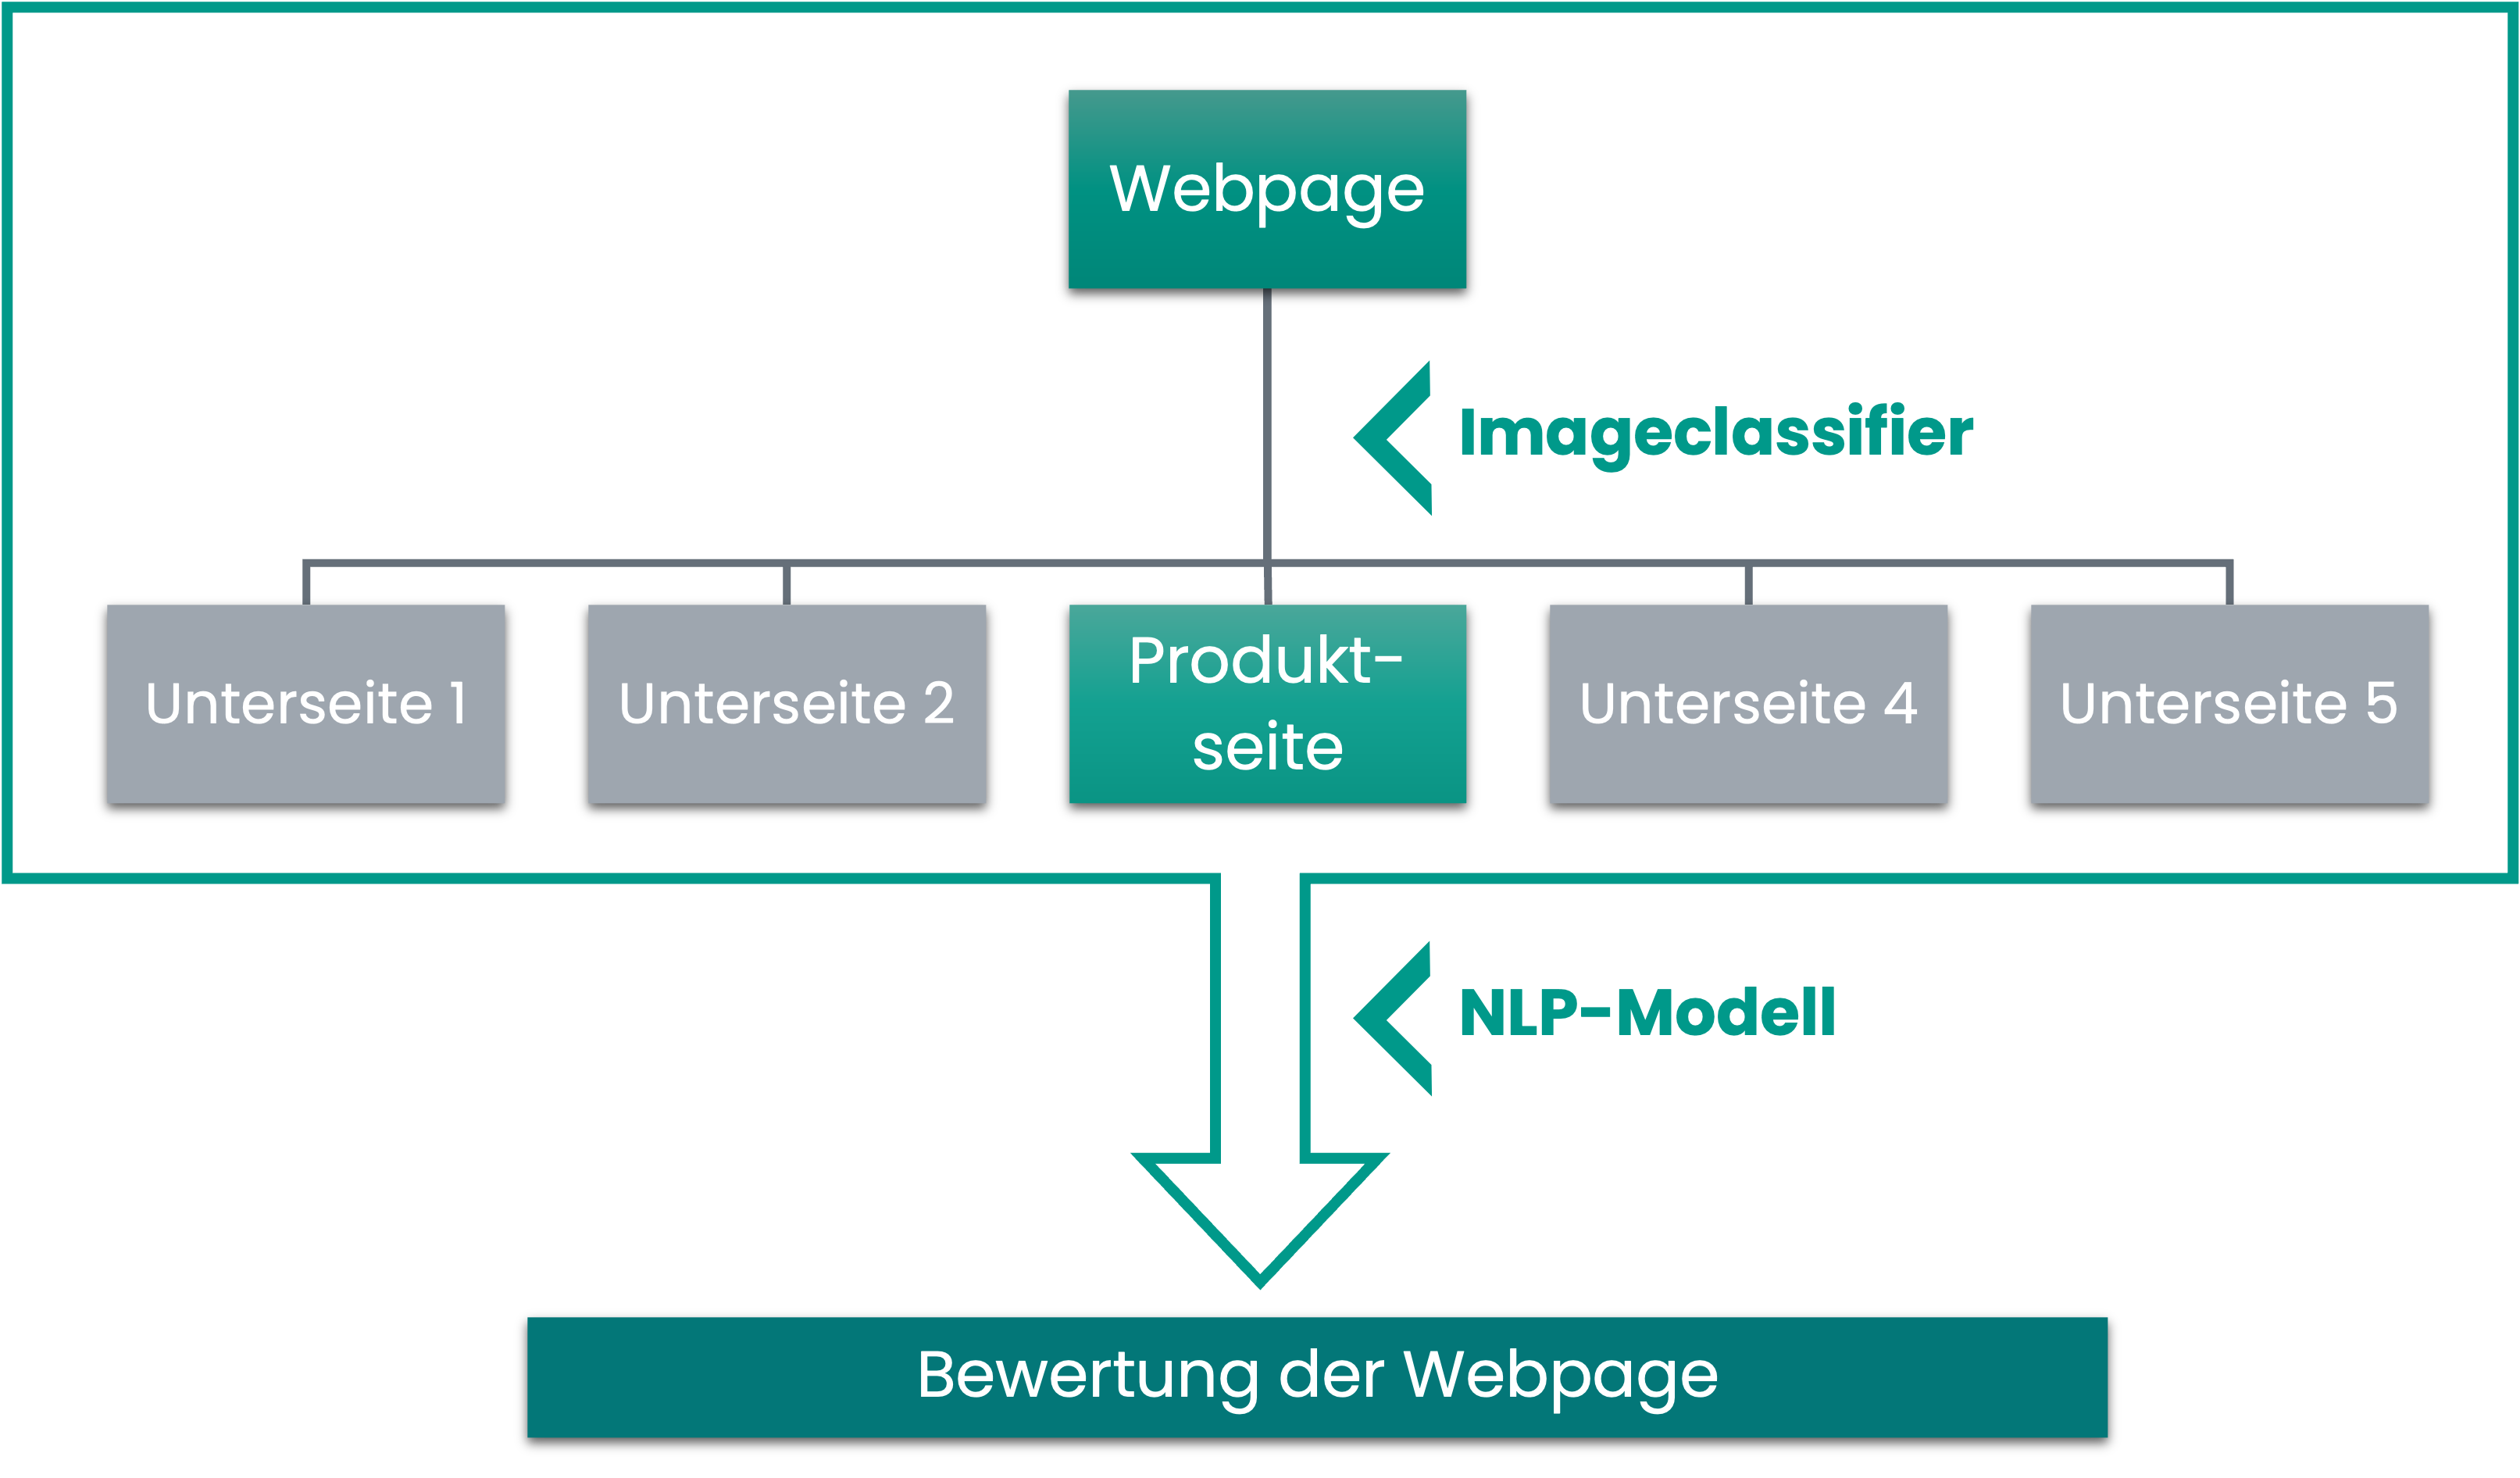
\includegraphics[width=0.9\textwidth]{zielbild.png}
	\\
	Quelle: Eigene Darstellung
\end{figure}

Um den OSMI-Index zu optimieren und zu automatisieren, wurde die in Abbildung~\ref{fig:zielbild} Pipeline aufgestellt mithilfe dessen
eine Website in Bezug auf den OSMI verarbeitet wird.
Der erste Schritt stellt dabei eine Vorverarbeitung der zu analysierenden Website dar, indem ein Image Classifier die Haupt- und Unterseiten der Website in
Produkt- und Nicht-Produktseiten unterteilt.
Dies ist aus Sicht der Autoren dieser Hausarbeit ein essenzieller Schritt, da so sichergestellt wird, dass die Bewertung des OSMI-Index lediglich auf Basis
der relevanten URLs vorgenommen wird.
Im darauf folgenden Schritt wird auf die textlichen Inhalte der relevanten Produktseiten ein \ac{NLP}-Modell angewendet, welches die Entitäten des OSMI-Index erkennt und auszählt.
Im abschließenden Schritt werden die Ergebnisse der Website-Analyse im Rahmen eines Dashboards visualisiert.
Nachfolgend wird die Umsetzung der soeben beschriebenen Schritte im Detail beschrieben und erläutert.

\subsection{Datenvorbereitung}

Sowohl in der Literatur als auch in bereits etablierten, gut entwickelten und veröffentlichten Modellen ist das Gebiet
des Sensory Marketings sehr rar vertreten.
Das bedeutet auch, dass im Hinblick auf den jüngst publizierten \ac{OSMI}-Index ebenfalls bisher wenig technische Entwicklungen
vorgenommen worden sind.
Zwar existieren in der Literatur diverse NLP-Modelle wie beispielsweise das generelle Spacy-Modell oder der sogenannte BERT
und von beiden erwähnten Modellen Spezialisierungen wie beispielsweise SciSpacy, BioBERT, ESG-BERT, etc\., allerdings ist
bisher kein NLP-Modell auf Marketingkontexte trainiert und publiziert worden, sodass die Notwendigkeit zur Entwicklung eines
eigenen Modells im Kontext des Consulting-Auftrags bestand.
Um im Vorfeld der Website-Bewertung jedoch lediglich nur die relevanten URLs mit Produktinhalt zu selektieren, wurde für den zu
entwickelnden Image Classifier ebenfalls ein von Grund auf neu zu entwickelndes Modell benötigt, da es innerhalb der Literatur
bislang kein derartig existierendes Modell publiziert wurde auf das zurückgegriffen werden konnte.

Die Trainingsdaten wurden mithilfe von Doccano generiert.
Doccano ist ein open source Tool, welches zur Annotation von Text und Bilddaten entwickelt wurde.
Mit diesem Instrument ist es also möglich Textpassagen und Bilder hochzuladen und Annotationen vorzunehmen, um Daten zur
Entwicklung von Aufträgen wie Named-Entity-Recognition, Textzusammenfassungen, Sentimentanalysen, Image Classification, etc.
zu generieren.

Im Rahmen des Consulting-Projekts wurden zwei Doccano-Projekte gestartet.
Ein Projekt wurde für das Annotieren von Textpassagen zur Entwicklung eines Named-Entity-Recognition Modells erstellt.
Im zweiten Projekt wurden Screenshots von Produktseiten und Nicht-Produktseiten annotiert.

Die Textpassagen, die annotiert wurden, sind im Rahmen des Consulting-Projekts zur Verfügung gestellt worden und entstammen
Webscraping-Ergebnissen von Vorgängerprojekten.
Hier wurden die fünf Sinne
\begin{itemize}
	\item Sight
	\item Smell
	\item Sound
	\item Taste
	\item Touch
\end{itemize}
als Label festgelegt und konnten im Rahmen des Annotationsprozesses ausgewählt werden.
Die in Abbildung~\ref{fig:annotation_ner} dargestellten horizontalen Balken geben den Annotationsstand wieder, auf Basis dessen
das Modell zur Erkennung von Entitäten entwickelt wurde.
Hier ist zu erkennen, dass die Entität \glqq{Sight}\grqq am häufigsten annotiert worden ist, während die Trainigs- und Testdaten für
die Entität \glqq{Smell}\grqq, \glqq{Sound}\grqq sowie \glqq{Taste}\grqq kaum vertreten sind.
\begin{figure}[H]
	\caption{Annotationsstand Textlabeling}\label{fig:annotation_ner}
	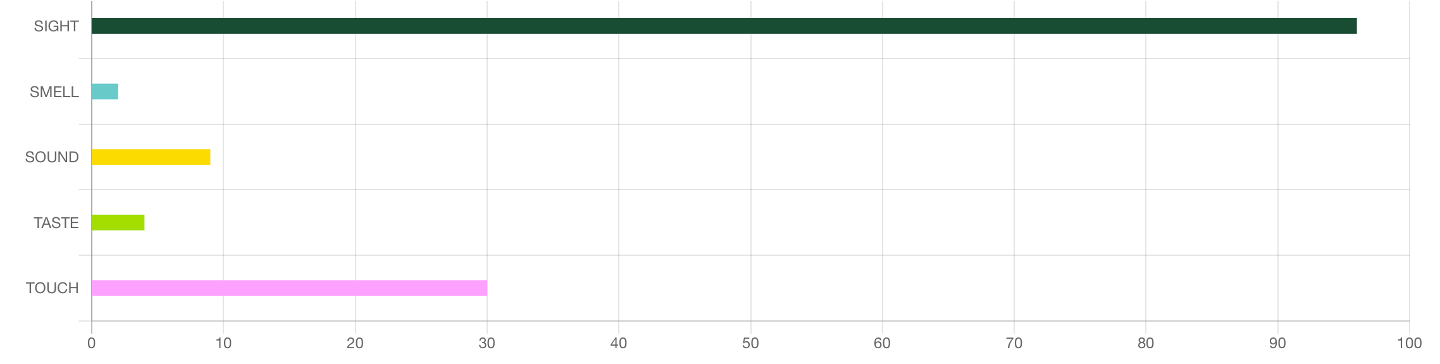
\includegraphics[width=0.9\textwith]{annotationen_ner.png}
	\\
	Quelle: Eigene Darstellung
\end{figure}

Die zu annotierenden Bilddaten von Produkt- und Nicht-Produktseiten wurden im Rahmen des behandelten Projektes selbständig
generiert.
Abbildung~\ref{fig:annotation_imgclf} zeigt, dass zur Modellentwicklung für den Image Classifier eine fast Gleichverteilung zwischen Produkt-
und Nicht-Produktseiten zugrunde gelegt wird.
Der Gesamtdatensatz beläuft sich auf rund 500 annotierten Bildern von Homepages.
\begin{figure}[H]
	\caption{Annotationsstand Textlabeling}\label{fig:annotation_imgclf}
	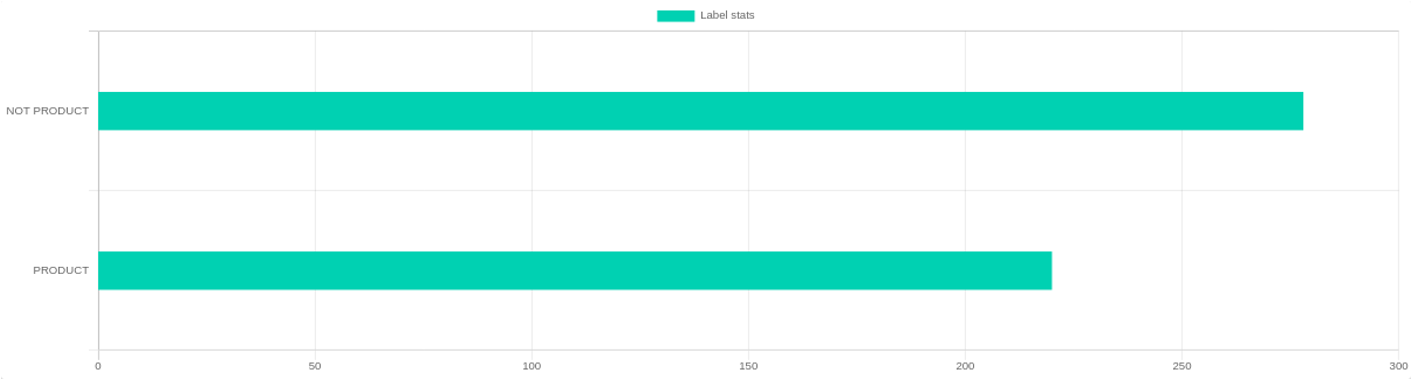
\includegraphics[width=0.9\textwidth]{annotationen_imgclf.png}
	\\
	Quelle: Eigene Darstellung
\end{figure}

\subsection{Modellentwicklung}
\subsubsection{NER-Modell}

\subsubsection{Image Classification Modell}